% %
% main.tex
%

% notes = hide | show | only
\documentclass[xcolor=dvipsnames,dvip,notes=show,table]{beamer}

% Para crear una versión 'handout' (impresa)
%\documentclass[xcolor=pst,dvips,handout,notes=show]{beamer}

%
% cabeceras.tex
%

\usepackage[T1]{fontenc}

 \definecolor{ZurichBlue}{rgb}{.255,.41,.884}
 \beamertemplateshadingbackground{white!10}{white!10}
%\usepackage{beamerthemeWarsaw}

% \usepackage{longtable}
\usepackage{beamerthemeBoadilla}


%\usepackage{tikz,times}
\usetheme{boxes}
%\usepackage{handoutWithNotes}
\usepackage{pgfpages}
%\pgfpagesuselayout{2 on 1}[a4paper,border shrink=5mm]


%\usecolortheme[named=OliveGreen]{structure} 
\setbeamertemplate{items}[ball] 
%\setbeamertemplate{blocks}[rounded][shadow=true] 
\setbeamertemplate{footline}[page number]
\addtocounter{framenumber}{-1}
%Handout



%\usepackage{beamertheme}
%\usepackage{beamerthemeshadow}
\useoutertheme[hooks]{tree}
 
% \setbeamertemplate{headline}[default] % The default is just an empty headline.
% \setbeamertemplate{headline}[infolines theme]
% \setbeamertemplate{headline}[miniframes theme]
% \setbeamertemplate{headline}[sidebar theme]
% \setbeamertemplate{headline}[smoothtree theme]
% \setbeamertemplate{headline}[smoothbars theme]
% \setbeamertemplate{headline}[tree]
\beamertemplatetransparentcovereddynamic
% spanish
\usepackage[spanish]{babel}
\usepackage[utf8]{inputenc}

% diagramas
%\usepackage{pst-eps,epstopdf}
\usepackage{pst-node}
%\usepackage{pst-all}
\usepackage{pst-blur}
%\usepackage{pst-tree}

% incrustaciones de código fuente
\usepackage{listings}

% matemáticas y símbolos
\usepackage{amsmath}
\usepackage{amssymb}
\usepackage[right]{eurosym}
\usepackage{ulem}

% colores
\usepackage{colortbl}

%\usepackage{algorithm2e}
%\usepackage{algorithm}
%\usepackage{algorithmic}

\lstset{language=[90]Fortran,
  basicstyle=\ttfamily,
  keywordstyle=\color{darkred},
  commentstyle=\color{green},
  frame=trBL,
  stringstyle=\color{violet},
  frameround=tttt,
  backgroundcolor=\color{lightyellow},
  morecomment=[l]{!\ }% Comment only with space after !
}


% 
% \lstset{%
%   language=Fortran,
% 	basicstyle=\footnotesize\sffamily,
% 	keywordstyle=\color{darkred}
%  	stringstyle=\color{violet}
%  	commentstyle=\color{blue}
%  	showspaces=false,
%  	showtabs=false,
%  	showstringspaces=false,
%  	frame=trBL,
%         frameround=tttt,
%         backgroundcolor=\color{lightyellow},
%  	extendedchars=true,
%  	numbers=none,
%         aboveskip=0.5cm,
%         belowskip=0.5cm,
%         xleftmargin=1cm,
%         xrightmargin=1cm,
% 	breaklines=true
% }
\definecolor{darkred}{rgb}{0.5, 0, 0}
\definecolor{violet}{rgb}{1, 0, 1}
\definecolor{lightyellow}{rgb}{1,1,0.8}


\usepackage{latexsym}
\usepackage{amsmath}
\usepackage{amssymb}
\usepackage{amsthm}

\usepackage{xspace}



\hyphenation{real}

\newrgbcolor{ColorEncabezadoTabla}{0.7 0.7 0.9}
\newrgbcolor{ColorFila1}{0.8 0.8 0.7}
\newrgbcolor{ColorFila2}{0.8 0.7 0.8}
\newrgbcolor{ColorTotal}{0.7 0.9 0.7}


% \usepackage{tikz,times}
% \usetikzlibrary{mindmap,backgrounds}
\usepackage{multirow}


%%%%%%%%%%%%%%%%%%%%%%%%%%%%%%%%%%%%%%%%%%%%%%%%%%%%%%%%%%%%%%%%%%%%%%

\title[The CORFU technique | MTSR 2013]{Towards a stepwise method for unifying and reconciling corporate names in public contracts metadata. \\ The CORFU technique.}
\author[Jose María Álvarez Rodríguez]{\textbf{Michalis Vafopoulos} (speaker) \\ and \\ \{Jose María Álvarez-Rodríguez, Patricia Ordoñez De Pablos and \\ Jose Emilio Labra-Gayo\}}
\institute{MTSR 2013 | 7th Metadata and Semantics Research Conference \\ Track on Metadata and Semantics for Open Repositories, Research Information Systems and Data Infrastructures}


\date{}

\begin{document}

\frame{
\titlepage

}

\frame{
\tableofcontents

}


\section{Introduction}

\frame{
  \frametitle{The Problem...What is the ``Big Name''?} 
  
\begin{table}[!htb]
\renewcommand{\arraystretch}{1.3}
\tiny
\begin{center}
\begin{tabular}{|p{7cm}|p{2cm}|}
\hline
  ``Oracle (Corp) Aust Pty Ltd''  & \multirow{11}{*}{``Oracle''} \\
 ``Oracle Corp (Aust) Pty Ltd''  &  \\
  ``Oracle Corp Aust Pty Ltd'' & \\
  ``Oracle Corp. Australia'' & \\
  ``Oracle Corp. Australia Pty.Ltd.'' & \\
  ``Oracle Corpoartion (Aust) Pty Ltd'' & \\
  ``Oracle Corporate Aust Pty Ltd'' & \\
  ``Oracle Corporation'' & \\
  ``Oracle Risk Consultants'' & \\
  ``ORACLE SYSTEMS (AUSTRALIA) PTY LTD'' & \\
  ``Oracle University''  & \\ 
  \ldots  & \\ \hline
   ``Accenture'' & \multirow{8}{*}{``Accenture''} \\
  ``Accenture Aust Holdings'' &  \\ 
   ``Accenture Aust Holdings'' & \\  
   ``Accenture Aust Holdings Pty Ltd'' & \\
   ``Accenture  Australia Holding P/L'' & \\
   ``Accenture Australia Holdings P/Ltd'' & \\
   ``Accenture Australia Holdings Pty Lt''  & \\  
  ``Accenture Australia Limited'' & \\
  \ldots  & \\ \hline
  \ldots & \ldots \\
  
  \hline
  \end{tabular}
\end{center}
\end{table} 

}

\frame{
  \frametitle{Scope}
  
  \begin{block}{Public Procurement}<1->
   \begin{enumerate}
    \item e-Procurement is a strategic sector (17\% of the GDP in Europe).
    \item Action Plans 2004 and 2020.
    \item Projects: E-Certis, Fiscalis 2013, E-Prior, PEPPOL, STORK,etc.
    \item Other actions: TED, RAMON metadata server, CPV, NUTS, etc.
    \item Legal Framework.
    \item Boost participation with special focus on SMEs.s
   \end{enumerate}
  \end{block}

   \begin{alertblock}{...but it also requires...}<2->
   \begin{enumerate}
    \item Accomplish with Open Data principles.
    \item Improve transparency of public bodies.
    \item Track where public money goes.
    \item \ldots
   \end{enumerate}
  \end{alertblock}
  
  
  }
  
\frame{
  \frametitle{The Problem...}
  
  \begin{block}{How can we track public procurement processes?}<1->
   \begin{enumerate}
    \item Data and information is already out there.
    \item Relevant metadata can be (re)used:
    \begin{itemize}
     \item Normalized product scheme classifications such as the CPV 2008 (Common Procurement Vocabulary).
     \item Territorial units (NUTS).
     \item Currency.
    \end{itemize}
    \item \ldots
   \end{enumerate}
  \end{block}
  
\begin{alertblock}{...and ``names''?}<2->
  Both \textbf{Payer} and \textbf{Payee} names are not usually normalized.
\end{alertblock}
  

\begin{block}{Normalized and unified names (``Big Name'')...}<3->
  ...with the aim of tracking both payers and payees.
\end{block}
   
  }

   
\frame{
  \frametitle{The Problem...}
  \begin{block}{Some remarks...}
   \begin{enumerate}
    \item It is \textbf{not} a mere problem of reconciling entities (dealing with)...
    \begin{itemize}
     \item Misspelling errors.
     \item Name/acronym mismatches.
     \item ...
    \end{itemize}
    \item ...but to c\textbf{reate a unique name or link }($n$ string literals $\to$ $1$ company $\to$ $1$ URI). 
    \item E.g.
    \begin{itemize}
     \item  ``Oracle'' and ``Oracle University'' could be respectively aligned to the entities $<$Oracle\_Corporation$>$ and $<$Oracle\_University$>$
     \item ...but the problem of grouping by a unique (\textit{Big}) name, identifier or resource still remains. 
    \end{itemize}
   \end{enumerate}

  \end{block}

  }

\section{Related Work}

\frame{
  \frametitle{Natural Language Processing and Computational Linguistics.} 
  \scriptsize
  \begin{block}{Existing works and APIs to deal with natural language issues}<1->
  \begin{enumerate}
 \item Misspelling errors~\cite{NorvigSpelling,StanfordSpelling}.
 \item Name/acronym mismatches~\cite{Yeates99automaticextraction}.
 \item APIs such as NLTK for Python, Lingpipe, OpenNLP or Gate for Java and search engines such as Apache Lucene/Solr.
 \item Extraction of clinical terms~\cite{Wang:2009:ARN:1667884.1667888} for electronic health records.
 \item Creation of bibliometrics~\cite{Galvez2006} or identification of gene names~\cite{Krauthammer:2004:TIB:1053007.1053018,Galvez2012}.
 \item \ldots
 \end{enumerate}
\end{block}

  
 \begin{alertblock}{Preliminary evaluation...}<2->
  \begin{itemize}
   \item Algorithms to deal with natural language hetereogenietes are already available.
   \item Existing works are usually focused in some domain (prototypes cannot be easily customized to other domain).
   \item ...but methodologies and NLP algorithms can be re-applied to new domains.
  \end{itemize}

 \end{alertblock}

 
 
}


\frame{
  \frametitle{Corporate Information.} 
  \scriptsize
  \begin{block}{Corporate Databases}<1->
  \begin{enumerate}
 \item Some corporate databases: The Spanish Chambers of Commerce, ``Empresia.es'' or ``Axesor.es'' to name a few (just in Spain).
 \item The DBPedia and the Orgpedia~\cite{Orgpedia}.
 \item The CrocTail~\cite{croctail} effort (part of the ``Corporate Research Project'').
 \item ``The Open Database Of The Corporate World''~\cite{Opencorporates}.
 \item Forbes, Google Places, Google Maps, Foursquare, Linkedin Companies or Facebook.
 \item \ldots
 \end{enumerate}
\end{block}

  
 \begin{alertblock}{Preliminary evaluation...}<2->
  \begin{itemize}
   \item Corporate information is public but access is restricted or under a fee (valuable metadata)...
   \item Large databases (``infobesity?'') but...
   \item ...the problem of mapping ,($n$ string literals $\to$ $1$ company $\to$ $1$ URI) as a human would do, still remains.
  \end{itemize}

 \end{alertblock}

 
 
}




\section{The CORFU technique}

\frame{
  \frametitle{Overview} 
}

\frame{
  \frametitle{Example} 
}

\frame{
  \frametitle{Step 1: FIXME} 
}


\subsection{Use Case: the Public Spending initiative}

\frame{
  \frametitle{Overview} 
}


\section{Evaluation and Discussion}

\frame{
  \frametitle{Research Design} 
  
  \begin{figure}[ht]
\begin{minipage}[b]{0.45\linewidth}
\centering
\begin{equation}\label{eq-1}
Precision = \frac{tp}{tp+fp} 
\end{equation}
\end{minipage}
\hspace{0.5cm}
\begin{minipage}[b]{0.45\linewidth}
\centering
\begin{equation}\label{eq-2}
Recall = \frac{tp}{tp+fn}
\end{equation}
\end{minipage}
\end{figure}


\begin{equation}\label{eq-3}
F1 = 2 \cdot \frac{Precision \cdot Recall}{ Precision + Recall}
\end{equation}



}

\frame{
  \frametitle{Results of applying the CORFU approach to the Australian supplier names.} 
  
  
\begin{table}[!h]
\renewcommand{\arraystretch}{1.3}
\scriptsize
\begin{center}
\begin{tabular}{|p{1.8cm}|p{1.3cm}|p{1.3cm}|p{1.3cm}|l|l|l|}
\hline
  \textbf{Total number of companies} & \textbf{Unique names}& \textbf{CORFU unified names}& \textbf{\% of unified names} & \textbf{Precision} & \textbf{Recall} & \textbf{F1 score} \\  \hline
   $430188$ & $77526$ & $40277$  &$48\%$ & $0.762$ & $0.311$&$0.441$ \\ \hline   
   $430188$ & $299$ in $77526$ & $68$ & $100\%$&  $0.926$ & $0.926$ &$0.926$\\ \hline
  \hline
  \end{tabular}
  %\caption{Results of applying the CORFU approach to the Australian supplier names.}
  \label{tabla:aus-results}
  \end{center}
\end{table} 

\scriptsize
\begin{exampleblock}{Comments}
 \begin{itemize}
  \item A $48\%$ ($77526-40278=37248$) of supplier names have been unified with a precision of $0.762$ and a recall of $0.311$ (best values must be close to $1$).
  \item The first 100 companies in the Forbes list, actually $68$ companies were found in the dataset with $299$ appearances.
  \item Results, in this second case, show a better performance: precision, $0.926$, and recall,$0.926$.
 \end{itemize}

\end{exampleblock}



  
  }


\frame{
  \frametitle{Graphical view of initial results without applying the CORFU technique...}
\begin{figure}[htb]
\centering
	
\includegraphics[width=6cm]{imgs/previous-corfu}
%\caption{Modelo $5\star$ (W3C).}
\end{figure}

  }
  

  \frame{
  \frametitle{Graphical view after applying the CORFU technique...}
\begin{figure}[htb]
\centering
	
\includegraphics[width=6cm]{imgs/corfu-stats}
%\caption{Modelo $5\star$ (W3C).}
\end{figure}

  }
  
  
  
  \frame{
  \frametitle{Graphical view after applying the CORFU technique to the first 100 Forbes companies...}
\begin{figure}[htb]
\centering
	
\includegraphics[width=6cm]{imgs/corfu-forbes-100}
%\caption{Modelo $5\star$ (W3C).}
\end{figure}

  }
  
  
    \frame{
  \frametitle{...the first 100 Forbes companies in bubbles...}
\begin{figure}[htb]
\centering
	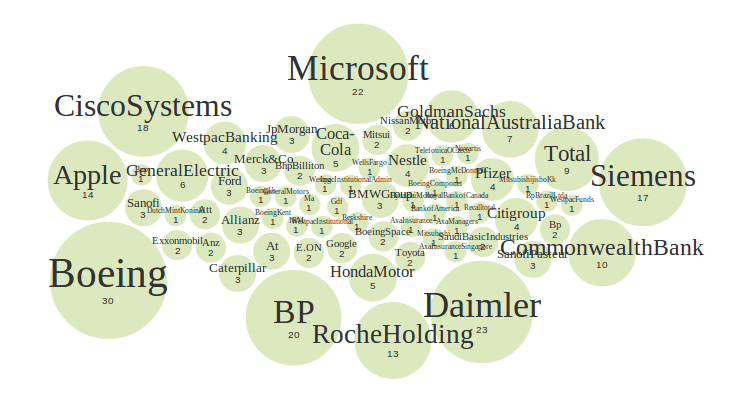
\includegraphics[width=10cm]{imgs/forbes}
%\caption{Modelo $5\star$ (W3C).}
\end{figure}

  }
  
  
  
\frame{
  \frametitle{Advantages} 
}


\frame{
  \frametitle{Restrictions} 
}



\section{Conclusions and Future Work}

\frame{
  \frametitle{Conclusions} 
}


\frame{
  \frametitle{Future Work} 
}




\section*{End of the presentation...}

\frame{
    
  \begin{figure}[!htb]
\centering
 
\includegraphics[width=9cm]{imgs/thanks}
\end{figure}


}



\section{Metadata and Information}


\frame{
  \frametitle{Roster...} 
  
  \begin{table}[!htb]

\scriptsize
\begin{center}
\begin{tabular}{p{3cm} p{7cm}}
  \begin{figure}[!htb]
\centering
 
\includegraphics[width=1cm]{imgs/chema}
\end{figure} & \begin{itemize}
                \item Dr. Jose María Alvarez-Rodríguez
                \item SEERC (until August, 2013) and Carlos III University of Madrid, Spain
                \item E-mail: \url{josemaria.alvarez@uc3m.es}
                \item WWW: \url{http://www.josemalvarez.es}
               \end{itemize} \\

\begin{figure}[!htb]
\centering
 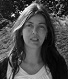
\includegraphics[width=1cm]{imgs/patriop}
\end{figure} & \begin{itemize}
                \item Prof. Dr. Patricia Ordoñez De Pablos
                \item University of Oviedo, Spain
                \item E-mail: \url{patriop@uniovi.es}
               \end{itemize} \\
               

\begin{figure}[!htb]
\centering
 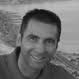
\includegraphics[width=1cm]{imgs/labra}
\end{figure} & \begin{itemize}
                \item Prof. Dr. Jose Emilio Labra-Gayo
                \item University of Oviedo, Spain
                \item E-mail: \url{labra@uniovi.es}
                \item WWW: \url{http://www.di.uniovi.es/~labra}
               \end{itemize}
               \end{tabular}
  \end{center}
\end{table} 

  
}



\appendix



\section*{References}
\bibliographystyle{abbrv}
\tiny
\bibliography{references}


% %%%%%%%%%%%%%%%%%%%%%%%%%%%%%%%%%%%%%%%%%%%%%%%%%%%%%%%%%%%%%%%%%%%%%%

\normalsize

\frame{
\titlepage

}

% %%%%%%%%%%%%%%%%%%%%%%%%%%%%%%%%%%%%%%%%%%%%%%%%%%%%%%%%%%%%%%%%%%%%%%

\end{document}
